\def\year{2019}\relax
%File: formatting-instruction.tex
\documentclass[letterpaper]{article} %DO NOT CHANGE THIS
\usepackage{aaai19}  %Required
\usepackage{times}  %Required
\usepackage{helvet}  %Required
\usepackage{courier}  %Required
\usepackage{url}  %Required
\usepackage{graphicx}  %Required
\frenchspacing  %Required
\setlength{\pdfpagewidth}{8.5in}  %Required
\setlength{\pdfpageheight}{11in}  %Required
\usepackage{float}

\usepackage[activate={true,nocompatibility},final,tracking=true,kerning=true,spacing=true,factor=1100,stretch=10,shrink=40]{microtype}

\makeatletter

% this creates a custom and simpler ruled box style
\newcommand\floatc@simplerule[2]{{\@fs@cfont #1 #2}\par}
\newcommand\fs@simplerule{\def\@fs@cfont{\bfseries}\let\@fs@capt\floatc@simplerule
  \def\@fs@pre{\hrule height.8pt depth0pt \kern4pt}%
  \def\@fs@post{\kern4pt\hrule height.8pt depth0pt \kern4pt \relax}%
  \def\@fs@mid{\kern8pt}%
  \let\@fs@iftopcapt\iftrue}

% this code block defines the new and custom floatbox float environment
\floatstyle{simplerule}
\newfloat{exmpl}{thp}{lob}[section]
\floatname{exmpl}{Example}


\usepackage{amssymb}
\usepackage{amsmath,amsthm}
\usepackage{float}
\usepackage{url}
\usepackage{setspace}
\usepackage{hyperref}
\usepackage{todonotes}
\usepackage{amsthm} 
\usepackage[ruled,vlined,linesnumbered]{algorithm2e} 
\usepackage{makecell}
\usepackage{upgreek}
\onehalfspacing
\usepackage{pdfpages}
\usepackage{times}
\usepackage{multirow}
\usepackage[toc,page]{appendix}
\usepackage{listings}
\newtheorem{thm}{Theorem}
\newtheorem{lemma}[thm]{Lemma}
\newtheorem{definition}[thm]{Definition}
\newtheorem{observation}[thm]{Observation}
\newtheorem{theorem}[thm]{Theorem}
\newtheorem{claim}[thm]{Claim}
\newtheorem{example}[thm]{Example}
\newtheorem{proposition}[thm]{Proposition}
\newtheorem{corollary}[thm]{Corollary}
\usepackage{color,soul}
\usepackage{tikz}
\usetikzlibrary{arrows,shapes.geometric,shapes.arrows}
\usepackage{pgfplots}
\usepackage{multirow}


\DeclareMathOperator{\supp}{support}
\DeclareMathOperator{\support}{support}
\DeclareMathOperator{\Trim}{Trim}
\DeclareMathOperator{\LTrim}{LTrim}
\SetKwFunction{mEqOne}{mEqOne} 
\DeclareMathOperator{\KlmApprox}{linApprox}
\DeclareMathOperator{\BinsApprox}{binsApprox}
\DeclareMathOperator{\OptTrim}{OptTrim}


  \pdfinfo{
	/Title (Efficient Optimal Approximation of Discrete Random Variables for Estimation of Probabilities of Missing Deadlines
	)
	/Author (Liat Cohen, Gera Weiss)}

\setcounter{secnumdepth}{1}  
\pgfplotsset{compat=1.5}
\begin{document}


\title{Efficient Optimal Approximation of Discrete Random Variables \\ for Estimation of Probabilities of Missing Deadlines}
\author{Liat Cohen \and Gera Weiss\\
    Department of Computer Science\\
		Ben-Gurion University of the Negev, Beer-Sheva 84105, Israel\\
		\{liati,geraw\}@cs.bgu.ac.il\\}
\maketitle
\begin{abstract}
We present an efficient algorithm that, given a discrete random variable $X$ and a number $m$, computes a random variable whose support is of size at most $m$ and whose Kolmogorov distance from $X$ is minimal. We present some variants of the algorithm, analyse their correctness and computational complexity, and present a detailed empirical evaluation that shows how they performs in practice. The main application that we examine, which is our motivation for this work, is estimation of the probability missing deadlines in series-parallel schedules. Since exact computation of these probabilities is NP-hard, we propose to use the algorithms described in this paper to obtain an approximation.   
\end{abstract}


\section{Introduction}


Various approaches for approximation of probability distributions are studied in the literature~\cite{PS77,AMCR83,vidyasagar2012metric,cohen2015estimating,pavlikov2016cvar,CohenGW18}. 
These approaches vary in the types random variables considered, how they are represented, and in the criteria used for evaluation of the quality of the approximations. In this paper we propose an approach for compressing the probability mass function of a random variable $X$ such that the errors added to queries such as $Pr(X\leq t)$, for  any $t>0$, is minimal. In other words, we minimise the Kolmogorov distance between the approximation and the original variable, see alternative definition in Equation~\eqref{eq:linear}. 

Our main motivation for this work is estimation of the probability for missing deadlines, as described, e.g., in Cohen et al.~\cite{cohen2015estimating,CohenGW18} and in~\cite{Kashef18}. Specifically, when $X$ represents the probability distribution of the time to complete some complex schedule and we cannot afford to maintain the full table of its probability mass function, we propose an algorithm for producing a smaller table, whose size can be specified, such that probabilities for missing deadlines are preserved as much as possible. 

The main contribution of this paper is an efficient algorithm for computing the best possible approximation of a given random variable with a random variable whose size is not above a prescribed threshold, where the measures of the quality of the approximation and of its size are as specified in the following two paragraphs. 

%The case study examined in this paper is the problem of task trees with deadlines~\cite{cohen2015estimating,CohenGW18}. A hierarchical plan is a method for representing problems of automated planning in which the dependency among tasks can be given in the form of networks, here we focus on hierarchical plans represented by task trees. The leaves in a task tree are \emph{primitive} actions (or tasks), and the internal nodes are either \emph{sequence} or \emph{parallel} actions. The plans we deal with are of stochastic nature, and the task duration is described as probability distributions in the leaf nodes. We assume that the distributions are independent but {\em not} necessarily identically distributed and that the random variables are discrete and have a finite support. 

%A sequence node denotes a series of tasks that should be performed consecutively, whereas a parallel node denotes a set of tasks that begin at the same time. A \emph{valid} plan is one that is fulfilled before some given \emph{deadline}, i.e., its \emph{makespan} is less than or equal to the deadline. The objective in this context is to compute the probability that a given plan is valid, or more formally computing $P(X<T)$, where $X$ is a random variable representing the makespan of the plan and $T$ is the deadline. The problem of finding the probability that a task tree satisfies a deadline is known to be NP-hard~\cite{cohen2015estimating}. In fact, even the problem of summing a set of random variables is NP-hard~\cite{mohring2001scheduling}. This is an example of an explicitly given random variable that we need to estimate deadline missing probabilities for.

We measure the quality of an approximation scheme by the distance between random variables and their approximations. Specifically, we use the Kolmogorov distance which is  commonly used for comparing random variables in statistical practice and literature. Given two random variables $X$ and $X'$ whose cumulative distribution functions (cdf) are $F_X$ and $F_{X'}$, respectively, the Kolmogorov distance between $X$ and $X'$ is $d_K(X,X')= \sup_t |F_X(t) - F_{X'}(t)|$ (see, e.g.,~\cite{gibbons2011nonparametric}). We say that $X'$ is a good approximation of $X$ if $d_K(X,X')$ is small. This distance is the basis for the often used Kolmogorov-Smirnoff test for comparing a sample to a distribution or two samples to each other. 

The size of a random variable is measured by the size of its support, the set of possible outcomes, $|X|{=}|\{x\colon Pr(X{=}x) \neq 0\}|$. When probability mass functions are maintained as tables, as done in many implementations of statistical software, the support size is proportional to the memory needed to store the variable and to the complexity of the computations that manipulate it. The exact notion of optimality of the approximation targeted in this paper is:

\begin{definition}
	A random variable $X'$ is an optimal $m$-approximation of a random variable $X$ if $|X'| \leq m$ and there is no random variable $X''$ such that $|X''| \leq m$ and $d_K(X,X'') < d_K(X,X')$.
\end{definition}

In these terms, the main contribution of the paper is an efficient (linear time and constant memory) algorithm that takes $X$ and $m$ as parameters and constructs an optimal $m$-approximation of $X$.

The rest of the paper is organised as follows. In Section~\ref{sec:relwork} we describe how our work relates to other algorithms and problems studied in the literature. In Section~\ref{sec:algEfficient} we detail the proposed algorithm, analyse its properties, and prove the main theorems. In Section~\ref{sec:exp} we demonstrate how the proposed approach performs on the problem of estimating the probability of missing deadlines in series-parallel schedules on randomly generated random variables and compare it to alternative approximation approaches from the literature. The paper is concluded with a discussion and with ideas for future work in Section~\ref{sec:discussion}.

%%%%%%%%%%%%%%%%%%%%%%%%%%%%%%%%%%%%%%%%%%%%%%%%%%%%%%%%%%%%%%%%%%%%%%%%%%%%%%%%%%%%%%%%%%%%
\section{Related work}\label{sec:relwork}
The most relevant work related to this paper is the papers on approximations of random variables in the context of estimating deadlines~\cite{cohen2015estimating,CohenGW18}. In these papers, $X'$ is defined to be a good approximation of $X$ if $F_{X'}(t) > F_{X}(t)$ for any $t$ and $\sup_t F_{X'}(t) - F_{X}(t)$ is small. Note that this measure is not a proper distance measure because it is not symmetric. The motivation given in these papers for using this type of approximation is for cases where overestimation of the probability of missing a deadline is acceptable but underestimation is not. We consider in this paper the same case-studies examined by Cohen et al. and show how the algorithm proposed in this paper performs relative to the algorithms proposed there when both over- and under- estimations are allowed. As expected, the Kolmogorov distance between the approximated and the original random variable is considerably smaller when using the algorithm proposed in this paper. 

In the technical level, the problem we study in this paper is similar to the problem of approximating a set of 2-D points by a step function. The study of this problem was motivated by query optimisation and histogram constructions in database management systems~\cite{applf12,applf13,applf14,applf17,applf18,Fournier2011} and computational geometry~\cite{diaz2001fitting,fournier2008fitting}. There are, however, two technically significant differences between the problem studied in the context of databases and the problem we analyse in this paper. The first difference is that in the context of approximation of random variables, the step function (which is the cumulative distribution function in our context)  must end with a value one, since we are dealing with random variables which sums to one. The second difference is that the first step is not counted because there is no need to put a value in the support of the approximated random variable to generate this first step. These cannot be addressed by adding a constant (two) to $m$ because the first step is always present and because the requirement to end with the value one, restricts the set of eligible step functions. 

Another relevant prior work is the theory of Sparse Approximation (aka Sparse Representation) that deals with sparse solutions for systems of linear equations, as follows. 
Given a matrix $D \in \mathbb{R}^{n \times p}$ and a vector $x \in \mathbb{R}^n$, the most studied sparse representation problem is finding 
%the sparsest possible representation $\alpha \in \mathbb{R}^p$ satisfying $x = D\alpha$:
$$
\min_{\alpha \in \mathbb{R}^p} \|\alpha\|_0 \text{ subject to } x = D\alpha
$$
where $\|\alpha\|_0 = |\{ i \in [p]: \alpha_i \neq 0 \}|$ is the $\ell_0$ pseudo-norm, counting the number of non-zero coordinates of $\alpha$. This problem is known to be NP-hard with a reduction to NP-complete subset selection problems.
In these terms, using also the $\ell_\infty$ norm that represents the maximal coordinate and the $\ell_1$ norm that represents the sum of the coordinates, our problem can be phrased as:
\begin{equation}\label{eq:linear}
\min_{\alpha \in [0,\infty)^p}\|x - D\alpha\|_{\infty} \text{ subject to }  \|\alpha\|_0 = m \text{ and } \|\alpha\|_1=1
\end{equation}
where $D$ is the lower unitriangular matrix, $x$ is related to $X$ such that the $i$th coordinate of $x$ is $F_X(x_i)$ where $\support(X)=\{x_1 < \cdots < x_n\}$ and $\alpha$ is related to $X'$ such that the $i$th coordinate of $\alpha$ is $f_{X'}(x_i)$. The functions $F_X$ and $f_{X'}$ represent, respectively, the cumulative distribution function of $X$ and the mass distribution function of $X'$, i.e.,  the coordinates of $x$ are positive and monotonically increasing and its last coordinate is one. %We show that this specific sparse representation problem can be solved in $O(n^2m)$ time and $O(m^2)$ memory.

The presented work is also related to the research on binning in statistical inference. Consider, for example, the problem of credit scoring~\cite{zeng2017comparison} that deals with separating good applicants from bad applicants where the Kolmogorov–Smirnov statistic KS is a standard measure. The KS comparison is often preceded by a procedure called binning where small values in the probability mass function are moved to nearby values. There are many methods for binning~\cite{mays2001handbook,refaat2011credit,bolton2010logistic,siddiqi2012credit}.
In this context, our algorithm can be considered as a binning strategy that provides optimality guarantees with respect to the Kolmogorov distance.

Our study is also related to the work of Pavlikov and Uryasev~\shortcite{pavlikov2016cvar}, where a procedure for producing a random variable $X'$ that optimally approximates a random variable $X$ is presented. Their approximation scheme, achieved using linear programming, is designed for a different notion of distance called CVaR. The contribution of the present work in this context is that our method is direct, not using linear programming, thus allowing tighter analysis of time and memory complexities. Also, our method is designed for minimising the Kolmogorov distance that is more prevalent in applications. For comparison, in Section~\ref{sec:exp} we briefly discuss the performance of linear programming approach similar to the one proposed in~\cite{pavlikov2016cvar} for the Kolmogorov distance and compare it our algorithm. 

A problem very similar to ours is termed ``order reduction'' by Vidyasagar in~\cite{vidyasagar2012metric}. There, the author defines an information-theoretic based distance between discrete random variables and studies the problem of finding a variable whose support is of size $m$ and its distance from $X$ is as small as possible (where $X$ and $m$ are given). The main difference between this and the problem studied in this paper, is that Vidyasagar examines a different notion of distance. Vidyasagar proves that computing the distance (that he considers) between two probability distributions, and computing the optimal reduced order approximation, are both NP-hard problems, because they can both be reduced to nonstandard bin-packing problems. He then develops efficient greedy approximation algorithms. In contrast, our study shows that there are efficient solutions to these problems when the Kolmogorov distance is considered. 

%%%%%%%%%%%%%%%%%%%%%%%%%%%%%%%%%%%%%%%%%%%%%%%%%%%%%%%%%%%%%%%%%%%%%%%%%%%%%%%%%%%%%%%%%%%%
\section{Algorithms for optimal approximation}\label{sec:algEfficient}
We begin with presenting an algorithm for solving a problem that is dual to the $m$-approximation problem: given a random variable $X$ and $0 \leq \varepsilon \leq 1$, find a new random variable $X'$ such that $d_k(X,X')\leq \varepsilon$ and $|X'|$ is minimal. 

We assume that the input to Algorithm~\ref{alg:dual} that solves the dual problem is a representation of the variable $X$ as a sorted CDF, i.e.,  as an array $X_{CDF}=\{(x_i, c_i)\}_{i=1}^n$ such that $c_i = Pr(X \leq x_i)$ and $\supp(X)=\{x_1 <\cdots < x_n\}$. In line~2 we perform a single pass over $X_{CDF}$ starting from the first index to find the last index where the cumulative distribution function of $X$ is less than $\varepsilon$, this index is stored in the variable $f$. In line 3 we start from the last index of $X_{CDF}$ which is $n$, and seek in decreasing order for the last index where the cumulative distribution function of $X$ is less than $1-\varepsilon$. This index is stored at the variable $l$. The last part of the algorithm is a pass on all elements of $X_{CDF}$ between the indices $f$ and $l$ in order to construct the random variable $X'$. In lines 6-7 we check if the difference between the first element in the current set of indices (which we call $b$) and the last element in the current set of indices (which we call $e+1$) is less than $2\varepsilon$. If yes, we add the pair $(x_{b}, (c_b+c_e)/2 - s)$ to the set $S$. Otherwise, we add one to $e$. See running Example~\ref{exmpl:dual}.

\begin{algorithm}
	\DontPrintSemicolon
	%Let $\{(x_i, c_i)\}_{i=1}^n$ be such that $c_i = Pr(X \leq x_i)$ and $\supp(X)=\{x_1 <\cdots < x_n\}$.\;
    $f \gets 1$, $l \gets n$+1\; 
    \lWhile{$c_{f} \leq \varepsilon$}{$f \gets f + 1$}

    \lWhile{$c_{l -1} \geq  1-\varepsilon$}{$l \gets l -1$}

	$S \gets \emptyset$, $s \gets 0$,$b \gets f$, $e \gets f$\;
	\While{$e<l$}{
	    \While{$c_{e+1}-c_{b} \leq 2\varepsilon \wedge e <l$}{$e \gets e+1$}
	    $S \gets S \cup \{(x_{b}, (c_b+c_e)/2 - s) \}$\;
        $s \gets  (c_b+c_e)/2$, $b \gets e\gets e+1$\;
	}
	$S \gets S \cup \{(x_{l}, 1 - s) \}$\;
    \Return{A r.v. $X'$ such that $Pr(X'{=}x)=c$ if there is $c$ such that $(x, c) \in S$ and $Pr(X'{=}x)=0$ otherwise.}
    	
    	
	
	\caption{$dual(\{(x_i, c_i)\}_{i=1}^n,\varepsilon)$  }   
	\label{alg:dual}
\end{algorithm}


\SetKwRepeat{Do}{do}{while}

\begin{example}
\label{exmpl:dual}
When $dual$ is invoked with the parameters  $X{=}\{(1, 0.3), (2, 0.7), (3, 0.9), (4,1)\}$ and $\varepsilon{=}0.1$: Lines 2 and 3 set $f=1$ and $l=4$. After an iteration of the main loop (line 5), $S = \{(1,0.3)\}$, $s=0.3$, and $b=e=2$. After a second iteration, $S = \{(1,0.3), (2, 0.5)\}$, $s=0.8$, and $b=e=4$. At the end, $S = \{(1,0.3), (2, 0.5), (4, 0.2)\}$.
\end{example}

\begin{proposition}\label{the:correctnessDual}
	If  $\{(x_i, c_i)\}_{i=1}^n$ is such that $c_i=Pr(X \leq x_i)$ and $\supp(X)=\{x_1 < \cdots < x_n\}$ then  
    $$dual(\{(x_i, c_i)\}_{i=1}^n,\varepsilon) \in \underset{X'\in \bar{\mathcal{B}}(X,\varepsilon)}{\operatorname{arg\,min}}\, |X'|$$  where $\bar{\mathcal{B}}(X,\varepsilon)=\{X'\colon d_K(X,X')\leq \varepsilon\}$.
\end{proposition}
\begin{proof}
The number of level sets of the CDF of $X'$ is minimal: (1) The first and the last sets are of maximal length; (2) By construction, an extension of any of the other sets to the right will generate a random variable whose Kolmogorov distance from $X$ is bigger than $\varepsilon$; and (3) Extension of a level set to the left may either leave the number of level sets unchanged or combine it with the previous set, which will enlarge the Kolmogorov distance because it is equivalent to extending the previous set to the right. Thus, there is no random variable whose Kolmogorov distance from $X$ is smaller or equal to $\varepsilon$ and its support is smaller than $|X'|$.
\end{proof}



\begin{proposition}\label{the:complexityDual}
	$dual(\{(x_i, c_i)\}_{i=1}^n,\varepsilon)$ runs in time $O(n)$, using $O(n)$ memory.
\end{proposition}
\begin{proof}
This algorithm describes a single pass over $\{(x_i, c_i)\}_{i=1}^n$. Lines 2 and 3 are easy to follow, each takes $O(n)$ in the worst case. Lines 5-9 also describe a single pass since the counter $e$ is updated to $e+1$ at most $n$ times. All together we get run-time complexity of $O(n)$. We are constructing the set $S$ which is of size $n$ in the worst case, therefore, memory complexity is $O(n)$. 
\end{proof}



The first solution to the $m$-approximation problem we present is the $binsApprox(X,m)$ algorithm which is based on~\cite{diaz2001fitting}. There are couple of significant changes between our $binsApprox(X,m)$ algorithm and the algorithm suggested by D{\'i}az-B{\'a}nez and Mesa~\shortcite{diaz2001fitting} addressing the differences presented in the Related work section. The algorithm $binsApprox(X,m)$ gets as input a random variable $X$ and some number $m$. Again, we do not mind the original representation of $X$ since we can transform it to a sorted CDF representation in $O(nlog(n))$ run-time as in line 1 which we call $X_{CDF}$. In lines 3-8 we compute all possible errors, in other words, all possible $d_{K}(X,X')$ such that $X'$ is an approximation of $X$ and $\support(X') \subseteq \support(X)$. The error is just the difference between the CDF values of every two elements in $X_{CDF}$. After computing the set $E$, we sort it (line 9) in order to perform a binary search. In lines 10-19 we perform a binary search over the set $E$, in every step of the binary search we run the $X' = dual(X,\varepsilon)$ algorithm. If the size of $|X'|>m$ then we know that the error $\varepsilon$ is too small and need to extend the search in the right side of $E$, if the size of $|X'|<m$ then we know that the error $\varepsilon$ is too big and need to extend the search in the left side of $E$, otherwise we found the correct $m$. 
We run the search twice to handle the extreme case where $m \notin \{|dual(X,\varepsilon)| \colon \varepsilon\in E \}$. In this case we may end up with a variable that is not optimal because it can be improved by using $m''$ such that $m < m'' < m'$. We find the optimal $m''$  by the second round ($i=2$) that run after line 18 that sets $m$ to be the $m'$ found in the first round.
 

\begin{algorithm}
	\DontPrintSemicolon
	Let $\{(x_i, c_i)\}_{i=1}^n$ be such that $c_i=Pr(X \leq x_i)$ and $\supp(X)=\{x_1 < \cdots < x_n\}$.\;
    $E \gets \emptyset$\; 
    \For{$i \gets 1$ \textbf{to} $n-1$}{
    	\For{$j \gets i+1$ \textbf{to} $n-1$}{
        		\If{$i=1$} {
                	$E \gets E \cup \{ c_j \}$
                }
        		$E \gets E \cup \{ (c_j-c_i)/2 \}$
        }
        $E \gets E \cup \{ 1 - c_i \}$
    }
    Let $e_1<\cdots<e_{n'}$ be such that $E=\{e_1,\dots,e_{n'}\}$ \;
    
    \For{$i \gets 1 \textbf{ to } 2$}{
        $l\gets 1$, $r \gets n'$, $k \gets 1$, $k' \gets 0$ \;
        \While{$k \neq k'$}{
                $k' \gets k$,$k \gets \lceil (l + r)/2 \rceil$\;
        		$m' \gets |dual(X,e_k)|$\;
        		\lIf{$m' < m$}{
        		    $l \gets k$
        		}
                \lIf{$m' > m$}{
        		    $r \gets k-1$
        		}
                \lIf{$m' = m$}{
        		    $r \gets k$
        		}
        }
        $m \gets m'$\;
    }
    \Return{$dual(X,e_k)$}

	\caption{$binsApprox(X,m)$}   
	\label{alg:naive}
\end{algorithm}


\begin{proposition}\label{the:correctnessBinsearch}
	    $binsApprox(X,m) \in \underset{|X'| \leq m }{\operatorname{arg\,min}}\, d_K(X,X')$
%     $binsApprox(X,m) \in \underset{X' \in \bar{\mathcal{B}}(X,m) }{\operatorname{arg\,min}}\, d_K(X,X')$ where $\bar{\mathcal{B}}(X,m)=\{X'\colon |X'| \leq m\}$.
\end{proposition}
\begin{proof}
Since lines 10-18 is a binary search of the smallest $e_k\in E$ such that $|dual(X,e_k)|\leq m$, we only need to prove that $E=E'=\{ d_K(X,dual(X,e_m)) \colon m=1,\dots,n\}$. To see that this is true, note that every element in $E'$ corresponds to a distance of a level set of the CDF of $dual(X,m)$ from the CDF of $X$ (because we seek a variable whose support is included in the original one). Line 6 of the algorithm adds all the distances from level sets of height zero, Line 8 adds the distances from level sets of height one, and Line 7 adds all the distances from all other possible level sets. Note that the distance is monotonic with the support size.
\end{proof}

\begin{proposition}\label{the:complexityBinsearch}
	The $binsApprox(X,m)$ algorithm runs in time $O(n^2log(n))$, using $O(n^2)$ memory where $n=|X|$.
\end{proposition}
\begin{proof}
	In the first part of the algorithm, lines 2-8, we construct the set $E$ which takes $O(n^2)$ run-time. In the second part of the algorithm, line 9, we sort the set $E$ which takes $O(n^2log(n^2)) = O(n^2log(n))$  run-time. The third part of the algorithm, lines 10-19, describes a binary sort over the set $E$ where in each step of the sorting we run the $dual$ algorithm, which takes $O(n log(n^2)) = O(n log(n))$ run-time. We run this part twice then we get $O(2n log(n))$. All together, the run-time complexity is $O(n^2+n^2log(n)+2n log(n)) = O(n^2log(n))$ and the memory complexity is for storing the set $E$ which is $O(n^2)$.
\end{proof}

Towards an improved algorithm let us introduce the matrix $E=(e_{i,j})_{i,j=1}^\infty$ defined by:
	$$e_{i,j} = \begin{cases}
	1-c_{n+1-j}   & \text{if } j \leq n \wedge  i = n ; \\
	c_i & \text{if } i \leq n \wedge  j = n + 1; \\
	( c_i - c_{n+1-j})/2  & \text{if } i < n \wedge j \leq n \wedge i{+}j\geq n; \\
	0  & \text{if }  i{+}j < n; \\
	1  & \text{otherwise}.
	\end{cases}$$
Where $c_1,\dots,c_n$ are as in the first line of Algorithm~\ref{alg:naive}. It is easy to see that the set of values in this matrix are the elements of the set $E$ in Algorithm~\ref{alg:naive}. An additional useful fact is that $E$ is a sorted matrix:
\begin{lemma}\label{the:sortedMatrix}
	If $i\leq i'$ and $j\leq j'$ then $e_{i,j}\leq e_{i',j'}$.
\end{lemma}
\begin{proof}
Since the $c_i$s are monotonically increasing, $\forall i,j$, $ 0\leq c_i - c_{n+1-j}\leq c_i - c_{n+1-(j+1)} $ and $ \forall i,j$, $0 \leq c_i - c_{n+1-j}\leq c_{i+1} - c_{n+1-j} $, moreover, 0 is the minimal value of $E$. The elements in the last row and the last column in $E$ are keeping the terms of sorted matrix. It suffices to compare row $n$ with row $n-1$ and show that $1-c_{n+1-j}\geq ( c_{n-1} - c_{n+1-j})/2$. After some manipulation we get that $2-c_{n+1-j}\geq c_{n-1}$ which is true because $0 \leq c\leq 1$. Next, it is suffice to compare column $n$ with only column $n+1$ and show that $c_i\geq ( c_{i} - c_{n+1-n})/2$. After some manipulation we get that $2c_i\geq c_{i}-c_1$ which is true because $0 \leq c_1 \leq c_i\leq 1$.
\end{proof}

The fact that this matrix is sorted allows us to use the saddleback search algorithm listed as Algorithm~\ref{alg:saddleback}. The algorithm starts at the top right entry of the matrix $(e_{i,j})_{i=1..n,j=1..(n+1)}$ and traverses it as follows. If it hits an entry $e$ such that $|dual(X,e)| \leq m$ it goes left, otherwise it goes down. This assures that the minimal $e$ such that $|dual(X,e)| \leq m$ is visited after at most $n+1$ steps. The optimal random variable is found by brute-force search over the visited entries.



\begin{algorithm}
	\DontPrintSemicolon
	Let $\{(x_i, c_i)\}_{i=1}^n$ be such that $c_i=Pr(X \leq x_i)$ and $\supp(X)=\{x_1 < \cdots < x_n\}$.\;
    $i \gets 1$, $j \gets n$+1, $S \gets \emptyset$\;

	\While{$i < n \wedge j \geq 1$}
	{	
		$m' \gets |dual(X,e_{i,j})|$\;
	
		\lIf {$m'  \leq m$}
		{
			$j \gets j - 1$
		}
		\lIf {$m' > m$} {
			$i \gets i + 1$
		}
		\lIf {$m' \geq m$} {
			$S \gets S \cup (m',e_{i,j})$			
		}

	}
	$e \gets \min\{e\colon (m',e) \in \underset{(m',e)\in S}{\operatorname{arg\,max}}\, m'\}$\;
	\Return{$dual(X,e)$}
	
	\caption{$sdlbkApprox(X,m)$}   
	\label{alg:saddleback}
\end{algorithm}


\begin{proposition}\label{the:correctnessSaddleback}
	   $sdlbkApprox(X,m) {\in} \underset{|X'| \leq m }{\operatorname{arg\,min}}\, d_K(X,X')$
%     $sdlbkApprox(X,m) {\in} \underset{X' \in \bar{\mathcal{B}}(X,m) }{\operatorname{arg\,min}}\, d_K(X,X')$ where $\bar{\mathcal{B}}(X,m)=\{X'\colon |X'| \leq m\}$.
\end{proposition}
\begin{proof}
The algorithm traverses all the frontier between those $e$s that satisfy $|dual(X,e)| \leq m$ and those that do not satisfy it. Since all the entries that satisfy the condition are recorded in $S$ and considered in the brute-force phase in line 7, the minimal satisfying $e$ is found.
\end{proof}

\begin{proposition}\label{the:complexitySaddleback}
	The $sdlbkApprox(X,m)$ algorithm runs in time $O(n^2)$, using $O(n)$ memory where $n=|X|$.
\end{proposition}
\begin{proof}
	At each step of the loop in lines 3-6, either $j$ decreases or $i$ increases, thus the loop can be executed at most $2n$ times. Since we execute $dual$ once in a loop round, the total time complexity is $O(n^2)$. Storing visited states in $S$ on line 6 requires  $O(n)$ memory.
\end{proof}

The problem with the saddleback algorithm is that it needs to run $dual$ at every step so it has a quadratic time complexity. Since we cannot find the required entry of the matrix in less than $n$ steps, we can only reduce the complexity by proposing an algorithm that does not execute $dual$ in all the steps, only in $\log(n)$ of them. Such an algorithm, based on Section~2.1 of~\cite{Fournier2011}, is listed as Algorithm~\ref{alg:linear}. The algorithm maintains a set $S$ of sub-matrices of $(e_{i,j})_{i=1..2^{\lceil \log_2(n) \rceil},j=1..2^{\lceil \log_2(n+1) \rceil}}$. At each round of its execution, each sub-matrix is split to four and then about three quarters of the matrix are discarded. At the end, at most four scalar matrices remain containing the index of the entry we seek. Note that this algorithm runs on a matrix that, in the worst case, can be almost four times bigger than the matrix traversed by the saddleback algorithm. This, of course, does not affect the asymptotic  complexity, but it may matter when dealing with relatively small random variables.

\begin{algorithm}
		\DontPrintSemicolon
		Let $\{(x_i, c_i)\}_{i=1}^n$ be such that $c_i=Pr(X \leq x_i)$ and $\supp(X)=\{x_1 < \cdots < x_n\}$.\;

		$S \gets  \{ ((1, 1),
		( 2^{\lceil \log_2(n) \rceil},2^{\lceil \log_2(n+1) \rceil})) \}$, $S' \gets \emptyset$\;
		
		
		\While{$S \neq S'$}
		{
			$S' \gets S$,
			$S \gets  \bigcup_{s \in S} split(s)$\;
			
			$e^- {\gets} median(\{ e_{i_1,j_1} \colon ((i_1,j_1),(i_2,j_2)) \in S \}) $\;		
			$e^+ {\gets} median(\{ e_{i_2,j_2} \colon ((i_1,j_1),(i_2,j_2)) \in S \}) $\;			

			\For{$ e \in \{ e^-,e^+ \}$} {
				$m' \gets |dual(X,e)|$\;
	
				\If {$m' \leq m$} {
					$S \gets$ $S \setminus \{ ((i_1,j_1),(i_2,j_2)) \in S \colon e_{i_1,j_1} > e \}$ \;
				}
			
				\Else %\If {$m'  > m$}
				{
					$S \gets$ $S \setminus \{ ((i_1,j_1),(i_2,j_2)) \in S \colon e_{i_2,j_2} \leq e \}$ \;
				}
			}
		}
	
		$S'' \gets \{(|dual(X,e_{i,j})|,e_{i,j}) \colon ((i,j),(i,j)) \in S\}$\;	
	
		$e \gets \min\{e\colon (m',e) \in \underset{(m',e)\in S''}{\operatorname{arg\,max}}\, m'\}$\;
		\Return{$dual(X,e)$}

		\caption{$linApprox(X,m)$}   
		\label{alg:linear}
	\end{algorithm}
{
	\begin{function}
		\DontPrintSemicolon
		
		$j^- \gets \lfloor (j_1+j_2)/2 \rfloor$,
		$j^+ \gets \lceil (j_1+j_2)/2 \rceil$\;
		$i^- \gets \lfloor (i_1+i_2)/2 \rfloor$,
		$i^+ \gets \lceil (i_1+i_2)/2 \rceil$\;

		\Return{\hspace{4cm}$
			\{ ((i_1, j_1), (i^-, j^-)),
			((i_1, j^+), (i^-, j_2))$,
			$((i^+, j_1), (i_2, j^-)),
			((i^+, j^+), (i_2, j_2))    \}$}
		
		\caption{{$split(((i_1,j_1),(i_2,j_2)))$}()}
		\label{proc:split}
	\end{function}
}	
	
	
\begin{theorem}\label{the:correctnessLinear}
	   
   $linApprox(X,m) {\in} \underset{|X'|\leq m}{\operatorname{arg\,min}}\, d_K(X,X')$
   
    % $linApprox(X,m) {\in} \underset{X' \in \bar{\mathcal{B}}(X,m) }{\operatorname{arg\,min}}\, d_K(X,X')$ where $\bar{\mathcal{B}}(X,m)=\{X'\colon |X'| \leq m\}$.
\end{theorem}
\begin{proof}
In line~10 we only discard sub-matrices whose minimal entry (at the top left) is larger than an entry that we prefer. In line~12 we only discard sub-matrices whose maximal entry (at the bottom right) is smaller or equal to an entry that does not meet our condition.
\end{proof}

\begin{theorem}\label{the:complexityLinear}
	The $linApprox(X,m)$ algorithm runs in time $O(n \log(n))$, using $O(1)$ memory where $n=|X|$.
\end{theorem}
\begin{proof}
The dimension of each matrix is halved in each round, thus the loop is executed $O(\log(n))$ rounds. Since $dual$ is called one in each round and a finite number of times at the end, the time complexity is $O(n \log(n))$.
\end{proof}

% \begin{example}\label{exmpl:dual}
% \small
% Let $X$ be such that $P(X {\leq} 1) {=} 0.333$, $P(X {\leq} 2) {=} 0.733$, $P(X {\leq} 3) {=} 0.9$, and $P(X{\leq} 4) {=} 1$ and $\varepsilon = 0.0833$. After lines 2, 3 of Algorithm~\ref{alg:dual}, $f{=}1$ and $l{=}4$. The first iteration (line 5) starts with $b{=}e{=}1$, and since $1{<}4$ we enter the first loop but not the second loop (line 6) because $0.733{-}0.333 {>} 0.166$. This iteration results with $S {=} \{(1,0.333)\}$, $s{=}0.333$, and $b{=}e{=}2$. In the second iteration we enter the first loop since $2{<}4$ and also the second loop because $0.9 {-} 0.7333 {\leq} 0.166$, and now $e{=}3$. Next we check if $1-0.733 {\leq} 0.166$ which is not true, therefore we exit the second loop. This iteration results with $S {=} \{(1,0.333), (2, 0.483)\}$, $s{=}0.816$, and $b{=}e{=}4$. The run ends with $S {=} \{(1,0.333), (2, 0.483), (4, 0.183)\}$. Note that the set $S$ represents the approximation random variable $X'$ whose support is of size 3 and the $d_K(X,X'){=}0.0833$.
% \end{example}


% \begin{example}[Dual algorithm running example]\label{exmpl:dual}
% Given the random variable $X$ in CDF representation: $P(X \leq 1) = 0.333, P(X \leq 2) = 0.733, P(X \leq 3) = 0.9, P(X\leq 4) = 1$ and some error $\varepsilon = 0.0833$. The dual algorithm first look for the range of $f$ and $l$.  In this example, after running lines 2, 3: $f=1$ and $l=4$. The first iteration (line 5) starts with $b=e=1$, and since $1<4$ we enter the first loop but not the second loop (line 6) because $0.733-0.333 > 0.166$. This iteration results with $S = \{(1,0.333)\}, s=0.333, b=e=2$. In the second iteration we enter the first loop since $2<4$ and also the second loop because $0.9 - 0.7333 \leq 0.166$, and now $e=3$. Next we check if $1-0.733\leq 0.166$ which is not true, therefore we exit the second loop. This iteration results with $S = \{(1,0.333), (2, 0.483)\}, s=0.816, b=e=4$. The run ends with $S = \{(1,0.333), (2, 0.483), (4, 0.183)\}$. Note that the set $S$ represents the approximation random variable $X'$ which his support is of size 3 and the $d_K(X,X')=0.0833$.
% \end{example}

\section{Experimental evaluation}\label{sec:exp}

We describe below several experiments that show how $\KlmApprox$ performs in practice in different applications and domains.
All algorithms were implemented in Python and the experiments were executed on a hardware comprised of an Intel i5-6500 CPU @ 3.20GHz processor and 8GB memory. The algorithms of Cohen et al. were taken ``as is" from in the supplementary material to~\cite{cohen2015estimating}.

\paragraph{Repetitive support size minimization.} One use of support size minimization is when commutations that involve summations of random variables slow due to an exponential growth in the support of convolutions of random variables~\cite{cohen2015estimating}. A key action in coping with this situation is reduction of the  support size by replacing the summed random variable by an approximation of it that has a smaller support size. Previous work such as the work of Cohen et al. in ~\shortcite{cohen2015estimating,CohenGW18} handle this reduction using weaker or sub-optimal notion of approximation than ours. 

As we proved above, given $m$, a single step of $\KlmApprox$ guarantees an optimal $m$-approximation. However in the setting considered here we need to repetitively use $\KlmApprox$, thus the optimality of the eventually obtained random variable is not guaranteed. In light of this, we tested the accuracy of the repetitive-$\KlmApprox$ to see how it performs against the tools of~\cite{cohen2015estimating,CohenGW18} using their benchmarks. These benchmarks are taken from the area of task trees with deadlines, a sub area of the well-established hierarchical planning~\cite{thomas1988hierarchical,alford2016hierarchical,xiao2017hierarchical}.

%The case study examined in our experiments is the problem of task trees with deadlines~\cite{cohen2015estimating,CohenGW18}. Hierarchical planning is a well-established field in AI~\cite{thomas1988hierarchical,erol1994htn,erol1996complexity}, and is still relevant nowadays~\cite{alford2016hierarchical,xiao2017hierarchical}. A hierarchical plan is a method for representing problems of automated planning in which the dependency among tasks can be given in the form of networks, here we focus on hierarchical plans represented by task trees. The leaves in a task tree are \emph{primitive} actions (or tasks), and the internal nodes are either \emph{sequence} or \emph{parallel} actions. The plans we deal with are of stochastic nature, and the task duration is described as probability distributions in the leaf nodes. We assume that the distributions are independent but {\em not} necessarily identically distributed and that the random variables are discrete and have a finite support. 


%A sequence node denotes a series of tasks that should be performed consecutively, whereas a parallel node denotes a set of tasks that begin at the same time. A \emph{valid} plan is one that is fulfilled before some given \emph{deadline}, i.e., its \emph{makespan} is less than or equal to the deadline. The objective in this context is to compute the probability that a given plan is valid, or more formally computing $P(X<T)$, where $X$ is a random variable representing the makespan of the plan and $T$ is the deadline. The problem of finding the probability that a task tree satisfies a deadline is known to be NP-hard. In fact, even the problem of summing a set of random variables is NP-hard~\cite{mohring2001scheduling}. This is an example of an explicitly given random variable that we need to estimate deadline meeting probabilities for.

%The first experiment we focus on is the problem of task trees with deadlines, and consider three types of task trees. The first type includes logistic problems of transporting packages by trucks and airplanes (from IPC2 http://ipc.icaps-conference.org/). Hierarchical plans of those logistic problems were generated by the JSHOP2 planner \cite{nau2003shop2}, one parallel node with all descendant task nodes being in sequence. 
%The second type consists of task trees used as execution plans for the ROBIL team entry in the DARPA robotics challenge (DRC simulation phase), and the third type is of linear plans (sequential task trees).
%The primitive tasks in all the trees are modeled as discrete random variables with support of size $M$ obtained by discretization of uniform distributions over various intervals. The number of tasks in a tree is denoted by $N$. 

We estimated the probability for meeting deadlines in plans, as described in Cohen et al.~\shortcite{cohen2015estimating,CohenGW18}, and experimented with four different methods of approximation. The first two, $\OptTrim$~\cite{CohenGW18} and the $\Trim$~\cite{cohen2015estimating}, are taken from the repository provided by the authors and are designed for achieving only a one-sided Kolmogorov approximation - a  weaker notion of approximation than the Kolmogorov approximation analyzed in this work. The third method is a simple sampling scheme and the fourth is our Kolmogorov approximation obtained by the proposed $\KlmApprox$ algorithm. The parameters for the different methods were chosen in a compatible way, $M$ is the maximal support size, $N$ is the number of nodes of the plan network and $s$ is the number of samples. We ran also an exact computation as a reference to the approximated one in order to calculate the errors. 

\begin{table}[th]
	\scriptsize
	\centering
	\renewcommand{\arraystretch}{1.3}
	\begin{tabular}{|p{1.05cm}|p{0.2cm}|p{0.98cm}|p{0.93cm}|p{1.05cm}|p{0.75cm}|p{0.75cm}|}
		\hline
		\multirow{2}{*}{Task Tree} & \multirow{2}{*}{$M$} & {$\KlmApprox$} & {$\OptTrim$} & {$\Trim$} & \multicolumn{2}{c|}{Sampling} \\ \cline{3-7} 
		&	& $m/N{=}10$ & $m/N{=}10$ & $\varepsilon\cdot N{=}0.1$ & $s{=}10^{4}$& $s{=}10^{6}$ \\ \hline
		\hline
		
		%N=34
		
		\multirow{2}{*}{Logistics} & 2& 0 & 0 &  0.0019 &  0.007 & 0.0009  \\ \Xcline{2-7}{1pt}
		{\tiny $(N=34)$}& 4& 0.0024 & 0.0046&  0.0068  &   0.0057 & 0.0005 \\\Xhline{1pt}
		
		%N=47
		\multirow{2}{*}{DRC-Drive}  
		&2	& 0.0014 & 0.004&  0.009  & 0.0072 & 0.0009  
		\\ \Xcline{2-7}{1pt}
		
		{\tiny $(N{=}47)$}& {4}& 0.001 & 0.008&  0.019   & 0.0075  & 0.0011 
		\\  \Xhline{1pt}
		
		
		%N=10
		\multirow{2}{*}{Sequential}  & {2} & 0.0093 & 0.015 &  0.024 & 0.0063 & 0.0008 \\ \Xcline{2-7}{1pt}  
		{\tiny $(N{=}10)$} & {4} & 0.008 & 0.024 &  0.04 & 0.008 & 0.0016 \\ \Xhline{1pt}
		
		
		
	\end{tabular}
	\caption{Comparison of estimated errors with respect to the reference exact computation on various task trees.}
	\label{tab:errors}
\end{table} 



Table~\ref{tab:errors} shows the results of the experiment. The quality of the solutions obtained with the $\KlmApprox$ operator are better than those obtained by the $\Trim$ and $\OptTrim$ operators as expected. In some of the task trees, the sampling method produced better results than $\KlmApprox$. Still, the $\KlmApprox$ approximation algorithm comes with an inherent advantage of providing exact quality guarantees, as opposed to sampling where the best one can hope for is probabilistic guarantees.

\paragraph{Run-time comparison.}
Similarly to accuracy and error computation, we also conducted empirical evaluation to examine the run-time in practice of the discussed algorithms. Figure~\ref{fig:runtime} presents a comparison of the run-time performances of an exact computation and approximated computations with $\KlmApprox$, $\BinsApprox$, $\OptTrim$ and $\Trim$ as operators. We examined four versions of approximation each of which with different run-time but only $\KlmApprox$ and $\BinsApprox$ produce optimal Kolmogorov approximation. The computation is a summation of a sequence of random variables with support size of $m{=}10$, where the number $n$ of variables varies from 6 to 19. In this experiment, we executed the approximation algorithm with $m{=}10$ after performing each convolution between two random variables, in order to maintain a support size of 10 in all intermediate computations. Equivalently, we executed the $\Trim$ operator with $\varepsilon=0.1$.
The results clearly show the exponential run-time of the exact computation, caused by the convolution between two consecutive random variables. In fact, in the experiment with $N{=}20$, the exact computation ran out of memory. These results illuminate the advantage of the proposed $\KlmApprox$ algorithm that balances between solution quality and run-time performance -- while there exist other, faster, methods (e.g., $\Trim$), $\KlmApprox$ provides high-quality solutions in $O(n log(n))$ time, which is especially important when an exact computation is not feasible, due to time or memory. In general, Figure~\ref{fig:runtime} is consistent with the theory and show a good fit to the complexity analysis. 


\begin{figure}[htb]
	\scriptsize	
	\centering 
	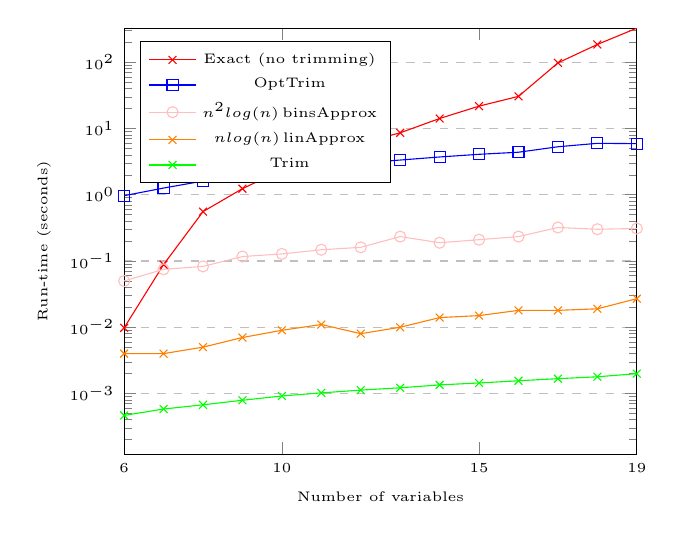
\begin{tikzpicture}
	\begin{axis}[
	scale=.95,
    ymode=log,
	xlabel={Number of variables},
	ylabel={Run-time (seconds)},
	xmin=6, xmax=19,
	%ymin=0, 
	ymax=327,
	xtick={6,10,15,19},
	legend pos=north west, style={font=\tiny\selectfont},
	ymajorgrids=true,
	grid style=dashed,
	]
	
	\addplot[
	color=red,
	mark=x,
	]
	coordinates {
		(6  , 0.00977492332458)
		(7  , 0.0880949497223)
		(8  , 0.556006193161)
		(9  , 1.23386096954)
		(10 , 2.37807798386)
		(11 , 4.2376730442)
		(12 , 6.03167200089)
		(13 , 8.61568593979)
		(14 , 14.1664741039)
		(15 , 21.7874569893)
		(16 , 30.5902190208)
		(17 , 97.9485061169)
		(18, 186.025614977) 
		(19, 327.884781122) 
	};
	\addlegendentry{Exact (no trimming)}

    \addplot[
	color=blue,
	mark=square,
	]
	coordinates { 
		(6 , 0.967791080475) 
		(7 , 1.26214194298) 
		(8 , 1.60830593109) 
		(9 , 1.97642302513) 
		(10, 2.28711390495) 
		(11, 2.67097711563) 
		(12, 3.01373195648) 
		(13, 3.3420279026) 
		(14, 3.71830201149) 
		(15, 4.08019995689) 
		(16, 4.3857190609) 
		(17, 5.30444002151)
		(18, 5.97745299339) 
		(19, 5.91222810745) 
	};
	\addlegendentry{$\OptTrim$}
	
    \addplot[
	color=pink,
	mark=o,
	]
	coordinates {
		(6  , 0.04986763000488281)
		(7  , 0.0747988224029541)
		(8  , 0.0827784538269043)
		(9  , 0.11668658256530762)
		(10 , 0.12765932083129883)
		(11 , 0.14760947227478027)
		(12 , 0.16057085990905762)
		(13 , 0.23337483406066895)
		(14 , 0.1884934902191162)
		(15 , 0.2094745635986328)
		(16 , 0.23337602615356445)
		(17 , 0.3201446533203125)
		(18, 0.3011953830718994) 
		(19, 0.3091733455657959) 
	};
	\addlegendentry{$n^2log(n) \BinsApprox$}
	
	\addplot[
	color=orange,
	mark=x,
	]
	coordinates {
		(6  , 0.003989458084106445)
		(7  , 0.00398707389831543)
		(8  , 0.004992485046386719)
		(9  , 0.006980419158935547)
		(10 , 0.008974790573120117)
		(11 , 0.010970354080200195)
		(12 , 0.007979631423950195)
		(13 , 0.00997161865234375)
		(14 , 0.013960838317871094)
		(15 , 0.014958381652832031)
		(16 , 0.017947673797607422)
		(17 , 0.017951011657714844)
		(18, 0.018949508666992188) 
		(19, 0.026926517486572266) 
	};
	\addlegendentry{$nlog(n) \KlmApprox$}
    
	
	\addplot[
	color=green,
	mark=x,
	]
	coordinates {
		(6  , 0.000465154647827)
		(7  , 0.000580787658691)
		(8  , 0.000672817230225)
		(9  , 0.000787973403931)
		(10 , 0.000914096832275)
		(11 , 0.00101804733276)
		(12 , 0.00112104415894)
		(13 , 0.0012149810791)
		(14 , 0.00134491920471)
		(15 , 0.00143694877625)
		(16 , 0.00155091285706)
		(17 , 0.00166893005371)
		(18 , 0.00178194046021)
		(19 , 0.00198793411255)
	};
	\addlegendentry{$\Trim$}
	\end{axis}
	\end{tikzpicture}
	\caption{Run-time of a long computation with $\KlmApprox$, $\BinsApprox$, $\OptTrim$, $\Trim$, and without any trimming.}
	\label{fig:runtime}
\end{figure}
\paragraph{Single step support minimisation.}
To better understand the quality gaps in practice between $\KlmApprox$, $\OptTrim$, and $\Trim$, we tested their performance on random variables with $n{=}100$, and different $m$s. Note that the error obtained by $\KlmApprox$ is optimal while the other methods are not optimised for the Kolmogorv distance. In each instance of the experiment, a random variable is randomly generated by choosing the probabilities of each element in the support uniformly and then normalise these probabilities to sum to 1.

Figure~\ref{fig:error} presents the error produced by the above methods. The depicted results are averages over fifty instances of random variables. The curves in the figure show the average error of $\OptTrim$ and $\Trim$ operators with comparison to the average error of the optimal approximation provided by $\KlmApprox$ as a function of $m$. It is evident from this graphs that increasing the support size of the approximation $m$ reduces the error, as expected, in all three methods. However, the errors produced by the $\KlmApprox$ are significantly smaller, a half of the error produced by $\OptTrim$ and $\Trim$.


\begin{figure}[htb]
	\scriptsize	
	\centering 
	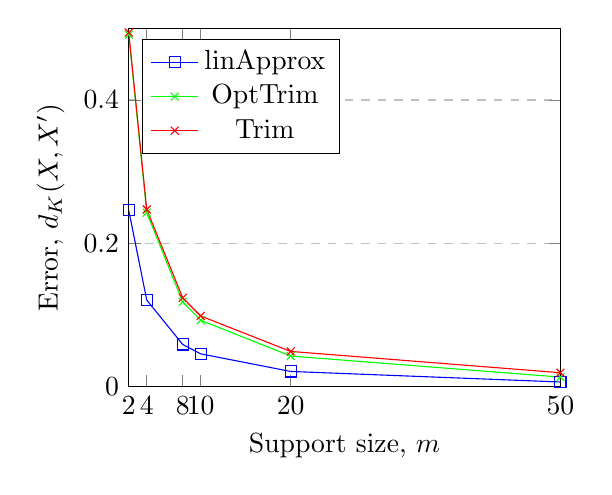
\begin{tikzpicture}
	\begin{axis}[
	scale=.8,
	xlabel={Support size, $m$},
	ylabel={Error, $d_K(X,X')$},
	xmin=2, xmax=50,
	ymin=0, ymax=0.5,
	xtick={2,4,8,10,20,50},
	legend pos=north west,
	ymajorgrids=true,
	grid style=dashed,
	]
	
	\addplot[
	color=blue,
	mark=square,
	]
	coordinates { 
		(2 , 0.246) 
		(4 , 0.121) 
		(8 , 0.0591) 
		(10 , 0.046) 
		(20, 0.0215) 
		(50, 0.0068) 
		
	};
	\addlegendentry{$\KlmApprox$}
	
	\addplot[
	color=green,
	mark=x,
	]
	coordinates {
		(2 , 0.491) 
		(4 , 0.2428) 
		(8 , 0.1184) 
		(10 , 0.0929) 
		(20, 0.0430) 
		(50, 0.0136) 
	};
	\addlegendentry{$\OptTrim$}
	
	\addplot[
	color=red,
	mark=x,
	]
	coordinates {
		(2 , 0.494) 
		(4 , 0.2473) 
		(8 , 0.124) 
		(10 , 0.0988) 
		(20, 0.0494) 
		(50, 0.01971)  
	};
	\addlegendentry{$\Trim$}
	
	\end{axis}
	\end{tikzpicture}
	\caption{Error comparison between $\KlmApprox$, $\OptTrim$, and $\Trim$ on randomly generated variables as function of $m$.}
	\label{fig:error}
\end{figure}

\paragraph{Comparison to Linear Programming.}
We also compared the run-time of $\KlmApprox$ with a linear programming (LP) algorithm that guarantees optimality, as described and discussed in~\cite{pavlikov2016cvar}.
We used the ``Minimize'' function of Wolfram Mathematica as a state-of-the-art implementation of linear programming, encoding the problem by the LP problem $\min_{\alpha \in \mathbb{R}^n} \| x - \alpha\|_\infty$ subject to $\|\alpha\|_0 \leq m$ and $\| \alpha \|_1{=}1$.
The run-time comparison results were clear and persuasive: $\KlmApprox$ significantly outperforms the LP algorithm. For a random variable with support size $n{=}10$ and $m=5$, the LP algorithm run-time was $850$ seconds, where the $\KlmApprox$ algorithm run-time was less than a second. For $n{=}100$ and $m{=}5$, the $\KlmApprox$ algorithm run-time was 0.14 seconds and the LP algorithm took more than a day. Since it is not trivial to formally analyze the run-time of the LP algorithm, we conclude by the reported experiment that in this case the LP algorithm might not be as efficient as $\KlmApprox$.

\section{Discussion and future work}\label{sec:discussion}
%Compact representations of distributions is mentioned in the literature in various contexts for various applications. In this paper, we are interested in finding optimal approximation of a random variables under the Kolmogorov metric which we define as optimal $m$-approximation. In order to achieve this optimal approximation two steps were taken, find the support of the optimal random variable and then calculate the pmf of each and every value in that support to minimize the error. Proofs of existences, optimality and run-time were detailed in Section~\ref{sec:alg} and the main algorithm was presented, the $\KlmApprox$ algorithm. Establishing the main contribution of this paper which is to present an optimal approximation scheme and to show it can be achieved in polynomial run-time. Furthermore, empirical evaluation was conducted on different domains and application to examine the algorithm performance in practice. We were interested in two aspects of performance - accuracy and run-time. Regarding to accuracy, as expected, the suggested $\KlmApprox$ algorithm results much smaller error compared to the other methods, sometimes, in more then factor 0f 2. Regarding to run-time, $\KlmApprox$ algorithm run-time is significantly much faster then LP approach. However, compared to other approximation methods accuracy vs. run-time is a trade off yet to be examined. Another interesting experiment that can be conducted in future work is to add the presented approach as one of the methods examined in~\cite{zeng2017comparison} and compare it to the binning approaches.

We developed an efficient algorithm for computing optimal approximations of random variables where the approximation quality is measured by the Kolmogorov distance.
As demonstrated in the experiments, our algorithm improves on the approach of Cohen et al.~\shortcite{cohen2015estimating} and~\shortcite{CohenGW18} in that it finds an optimal two sided Kolmogorov approximation, and not just one sided. In addition, the algorithm $\KlmApprox$ presented in this paper is very efficient with complexity of $O(n log(n))$ as proved in Theorem~\ref{the:complexityLinear} and showed in Figure~\ref{fig:runtime}. Beyond the Kolmogorov measure studied here, we believe that similar approaches may apply also to total variation, to the Wasserstein distance, and to other measures of approximations. %Another direction for future work is extensions to tables that represent other objects, not necessarily random variables. To this end, we need to extend the algorithm to support tables that do not always sum to one and tables that may contain negative entries.

%\begin{example}
%Given $m=3$ and the random variable $X$ in CDF representation: $P(X \leq 1) = 0.3333, P(X \leq 2) = 0.7333, P(X \leq 3) = 0.9, P(X\leq 4) = 1$. Find an approximation of $X$ with support of size 3. First step, find all differences: $E= \{0, 0.05, 0.0833, 0.1, 0.133, 0.2, 0.266, 0.2833, 0.333, 0.666,\\ 0.7333, 0.9, 1\}$. Next, perform a binary search over $E$, in order to compute the dual support size. Starting with $E[7] = 0.266$ results with support size of 2, therefore, we adjust the search to smaller $E$ values, in this case $E[3] =  0.0833$ where the dual support size is 3. Even though $m=3$, we also seek for optimal (minimal) error, leading to check $e[2]=0.05$ as well which produce dual support size of 4. Therefore, we know $\varepsilon =  0.0833$ is the optimal error for $m=3$.
%\end{example}

\paragraph{Acknowledgments.} This research was supported by the Lynn and William Frankel Centre for Computer Science at Ben-Gurion University and by the Israel Science Foundation.

\bibliographystyle{aaai}
\bibliography{library,Trim_Optimum}


\end{document}
